%&LaTeX
% !TEX encoding = UTF-8 Unicode

%Borrowed from ADIOS Manual, may be some unneccesary bits here...

\documentclass{report}
\usepackage[utf8]{inputenc}
\usepackage[T1]{fontenc}
\usepackage{textcomp}
\usepackage{float,fancyvrb}
\usepackage{listings}

%\usepackage{graphicx}
\usepackage{longtable}
\usepackage{color}

\usepackage{ifpdf}

\ifx\pdftexversion\undefined %if using TeX
    \usepackage{graphicx}
\else %if using PDFTeX
    \ifpdf %if using PDFTeX in PDF mode
        \usepackage[pdftex]{graphicx}
        \DeclareGraphicsExtensions{.pdf,.png,.mps}
        \usepackage{pgf}
    \else %if using TeX or PDFTeX in TeX mode
        \usepackage{graphicx}
        \DeclareGraphicsExtensions{.eps,.bmp}
        \DeclareGraphicsRule{.emf}{bmp}{}{}% declare EMF filename extension
        \DeclareGraphicsRule{.png}{bmp}{}{}% declare PNG filename extension
        \usepackage{pgf}
        \usepackage{pstricks} %variant: \usepackage{pst-all}
\fi

%\setlength{\paperheight}{297mm}
%\setlength{\paperwidth}{210mm}
%\setlength{\voffset}{11mm}
\setlength{\topmargin}{0mm}
\setlength{\headsep}{0mm}
\setlength{\headheight}{0mm}
\setlength{\textheight}{235mm}
\setlength{\hoffset}{-4mm}
\setlength{\textwidth}{166mm}
\setlength{\oddsidemargin}{0mm}
\setlength{\evensidemargin}{0mm}
\setlength{\marginparwidth}{0mm}
\setlength{\marginparpush}{0mm}
%\setlength{\columnsep}{6mm}
%\setlength{\parindent}{0mm}


\definecolor{color01}{rgb}{0.00,0.00,0.00}
\definecolor{color02}{rgb}{0.00,0.00,1.00}
\definecolor{color06}{rgb}{1.00,0.00,0.00}
\definecolor{color08}{rgb}{1.00,1.00,1.00}
\definecolor{color17}{rgb}{0.14,0.25,0.38}
\definecolor{color20}{rgb}{0.31,0.51,0.74}
\definecolor{color26}{rgb}{0.50,0.50,0.50}

%% Added by Jong -- to enable \subsubsection
\setcounter{secnumdepth}{3}
\usepackage{hyperref}

\newcommand{\comment}[1]{}

%%%%%%%%%%%%%%%%%%%%%%%%%%%%%%%%%%%%%%%%%%%%%%%%%%%%%%%%%%%%%%%%%%%%%%%
% Define syntax highlighting for ADIOS
\lstdefinelanguage{ADIOS}
{
sensitive=true,
keywordsprefix=ADIOS_,
morekeywords=[1]{
adios_errno, err_file_not_found, err_end_of_stream, err_step_notready, err_step_deleted},
morekeywords=[2]{
% Write API (XML)
adios_init, adios_finalize, adios_open, adios_write, adios_read, adios_close, 
adios_group_size, adios_set_path_var, adios_set_path, 
adios_end_iteration, adios_start_calculation, adios_stop_calculation,
% Write API (Non-XML)
adios_init_noxml, adios_declare_group, adios_free_group, adios_define_var, 
adios_define_attribute, adios_allocate_buffer, adios_select_method,
adios_get_write_buffer,
% Read API (1.4)
adios_read_init_method, adios_read_finalize_method,
adios_read_open_file, adios_read_open, adios_read_close,
adios_inq_var, adios_inq_var_byid, adios_free_varinfo,
adios_inq_var_stat, adios_inq_var_blockinfo,
adios_get_attr, adios_get_attr_byid,
adios_schedule_read, adios_schedule_read_byid, adios_perform_reads, adios_check_reads,
adios_advance_step, adios_release_step,adios_free_chunk,
adios_selection_boundingbox, adios_selection_points, adios_selection_writeblock, 
adios_selection_delete, adios_selection_auto, adios_errmsg,
adios_type_to_string, adios_type_size, adios_get_grouplist,
% Fortran Read
adios_reset_dimension_order, adios_inq_ngroups, adios_inq_groupnames, 
adios_group_view, adios_inq_file, adios_inq_varnames, adios_inq_attrnames,
adios_inq_attr, adios_get_scalar, adios_get_statistics},
morecomment=[l]{//},morecomment=[s]{/*}{*/},
morestring=[b]",morestring=[b]',
}

\lstdefinelanguage{cython}[]{python}
{
sensitive=true,
keywordsprefix=ADIOS_,
keywords={def, cpdef, cdef, public, class, self},
morekeywords=[1]{
int64_t, uint64_t, int, long, float, double, char, bytes, tuple, list, dict},
upquote=true,
}

\lstdefinelanguage{ADIOS-python}[]{python}
{
upquote=true,
}

\definecolor{gray}{rgb}{0.35,0.35,0.35}
\definecolor{gray85}{rgb}{0.85,0.85,0.85}
\definecolor{javared}{rgb}{0.6,0,0}
\definecolor{javagreen}{rgb}{0.25,0.5,0.35}
\definecolor{javapurple}{rgb}{0.5,0,0.35}
\definecolor{javadocblue}{rgb}{0.25,0.35,0.75}

\lstset{language=ADIOS, basicstyle=\ttfamily, numbers=none,
  showspaces=false, showstringspaces=false,
  keywordstyle=[1]\color{javapurple},
  keywordstyle=[2]\color{blue}\bf,
  stringstyle=\color{javared},
  commentstyle=\color{javagreen},
  captionpos=b,
  frame=no,
  escapechar=`,
}
% End of syntax highlight def for ADIOS
%%%%%%%%%%%%%%%%%%%%%%%%%%%%%%%%%%%%%%%%%%%%%%%%%%%%%%%%%%%%%%%%%%%%%%%

\begin{document}


\vspace{24pt}
\begin{flushright}
{\color{color08} \textbf{ORNL/TM-2009/100\label{OLEHLINK6}}}
\end{flushright}

\vspace{60pt}
{\huge \textbf{ADIOS 1.5.0 Developer's Manual}}

\vspace{36pt}
\textbf{July 2012\pagebreak{}}


\begin{longtable}{|p{4.443in}|p{0.057in}|}
\hline

\begin{center}
{\small \textbf{DOCUMENT AVAILABILITY}}
\end{center}


{\small Reports produced after January 1, 1996, are generally available free via 
the U.S. Department of Energy (DOE) Information Bridge:}


\leftskip=18pt
{\small \textbf{Web site:}}{\small  http://www.osti.gov/bridge}


\leftskip=0pt
{\small Reports produced before January 1, 1996, may be purchased by members of 
the public from the following source:}


\parindent=18pt
{\small National Technical Information Service}

{\small 5285 Port Royal Road}

{\small Springfield, VA 22161}

{\small \textit{\textbf{Telephone:}}}{\small  703-605-6000 (1-800-553-6847)}

{\small \textit{\textbf{TDD:}}}{\small  703-487-4639}

{\small \textit{\textbf{Fax:}}}{\small  703-605-6900}

{\small \textit{\textbf{E-mail:}}}{\small  info@ntis.fedworld.gov}

{\small \textit{\textbf{Web site:}}}{\small  http://www.ntis.gov/support/ordernowabout.htm}


\parindent=0pt
{\small Reports are available to DOE employees, DOE contractors, Energy Technology 
Data Exchange (ETDE) representatives, and International Nuclear Information System 
(INIS) representatives from the following source:}


\parindent=18pt
{\small Office of Scientific and Technical Information}

{\small P.O. Box 62}

{\small Oak Ridge, TN 37831}

{\small \textit{\textbf{Telephone:}}}{\small  865-576-8401}

{\small \textit{\textbf{Fax:}}}{\small  865-576-5728}

{\small \textit{\textbf{E-mail:}}}{\small  reports@adonis.osti.gov}

\leftskip=18pt
\parindent=0pt
{\small \textit{\textbf{Web site:}}}{\small  http://www.osti.gov/contact.html}

\\\hline
\end{longtable}

%\vspace{48pt}
\begin{longtable}{|p{4.443in}|p{0.057in}|}
\hline
% ROW 1
\begin{minipage}[t]{4.443in}\raggedright %\linebreak
{\small This report was prepared as an account of work sponsored by an agency of 
the United States Government. Neither the United States government nor any agency 
thereof, nor any of their employees, makes any warranty, express or implied, or 
assumes any legal liability or responsibility for the accuracy, completeness, or 
usefulness of any information, apparatus, product, or process disclosed, or represents 
that its use would not infringe privately owned rights. Reference herein to any 
specific commercial product, process, or service by trade name, trademark, manufacturer, 
or otherwise, does not necessarily constitute or imply its endorsement, recommendation, 
or favoring by the United States Government or any agency thereof. The views and 
opinions of authors expressed herein do not necessarily state or reflect those 
of the United States Government or any agency thereof.}\end{minipage}\\
\hline
\end{longtable}
\pagebreak{}

\vspace{12pt}
\begin{flushright}
{\color{color08} \textbf{ORNL/TM-2009/100\label{HToc533553247}\label{HToc6041549}\label{HToc6042388}\label{HToc8548020}\label{HToc528144461}\label{HToc528743868}\label{HToc528745033}}}
\end{flushright}

%\vspace{36pt}
\begin{center}
{\Large \textbf{ADIOS 1.5.0 DEVELOPER'S MANUAL}}

\vspace{60pt}
Prepared for the

%\vspace{12pt}
Office of Science

%\vspace{12pt}
U.S. Department of Energy

\vspace{60pt}
Authors

\vspace{6pt}
N. Podhorszki, Q. Liu, J. Logan, H. Abbasi, J.Y. Choi, S. Klasky

\vspace{30pt}
Contributors 

\vspace{6pt}
J. Lofstead, S. Hodson, F. Zheng, M. Wolf, T. Kordenbrock, N. Samatova

\vspace{72pt}
July 2012

\vspace{72pt}
Prepared by

%\vspace{24pt}
OAK RIDGE NATIONAL LABORATORY

%\vspace{12pt}
Oak Ridge, Tennessee 37831-6070

%\vspace{12pt}
managed by

%\vspace{12pt}
UT-BATTELLE, LLC

%\vspace{12pt}
for the

%\vspace{12pt}
U.S. DEPARTMENT OF ENERGY

%\vspace{12pt}
under contract DE-AC05-00OR22725

%\vspace{42pt}
\end{center}


\newpage

\tableofcontents


\newpage

\listoffigures


\newpage


\vspace{66pt}
\textbf{Abbreviations}

\begin{description}
\item[ADIOS]  Adaptive Input/Output System
\item[API] Application Program Interface
\item[DART] Decoupled and Asynchronous Remote Transfers
\item[GTC] Gyrokinetic Turbulence Code
\item[HPC] High-Performance Computing
\item[I/O] Input/Output
\item[MDS] Metadata Server
\item[MPI] Message Passing Interface
\item[NCCS] National Center for Computational Sciences
\item[ORNL] Oak Ridge National Laboratory
\item[OS] Operating System
\item[PG] Process Group
\item[POSIX] Portable Operating System Interface
\item[RDMA] Remote Direct Memory Access
\item[XML] Extensible Markup Language
\end{description}


\vspace{18pt}
\begin{center}
{\large \textbf{Acknowledgments}}
\end{center}

\vspace{6pt}
This project is sponsored by ORNL, Georgia Tech, The Scientific Data Management 
Center (SDM) at Lawrence Berkeley National Laboratory, and the U.S. Department 
of Defense. 



\chapter{Introduction}

\section{Goals}

%\leftskip=0pt
%\parindent=0pt
As computational power has increased dramatically with the increase in the number
of processors, input/output (IO) performance has become one of the most significant
bottlenecks in today's high-performance computing (HPC) applications. With this
in mind, ORNL and the Georgia Institute of Technology's Center for Experimental
Research in Computer Systems have teamed together to design the Adaptive I/O System
(ADIOS) as a componentization of the IO layer, which is scalable, portable, and
efficient on different clusters or supercomputer platforms. We are also providing
easy-to-use, high-level application program interfaces (APIs) so that application
scientists can easily adapt the ADIOS library and produce science without diving
too deeply into computer configuration and skills.

\section{What is ADIOS?}

{\color{color01} ADIOS is a state-of-the-art componentization of the IO system
that has demonstrated impressive IO performance results on leadership class machines
and clusters; sometimes showing an improvement of more than 1000 times over well
known parallel file formats. }ADIOS is essentially an I/O componentization of different
I/O transport methods. This feature allows flexibility for application scientists
to adopt the best I/O method for different computer infrastructures with very little
modification of their scientific applications. ADIOS has a suite of simple, easy-to-use
APIs. Instead of being provided as the arguments of APIs, all the required metadata
are stored in an external Extensible Markup Language (XML) configuration file,
which is readable, editable, and portable for most machines.

\section{The Basic ADIOS Group Concept}

The ADIOS ``group'' is a concept in which input variables are tagged according
to the functionality of their respective output files. For example, a common scientific
application has checkpoint files prefixed with restart and monitoring files prefixed
with diagnostics. In the XML configuration file, the user can define two separate
groups with tag names of adios-group as ``restart'' and ``diagnostic.'' Each group
contains a set of variables and attributes that need to be written into their respective
output files. Each group can choose to have different I/O transport methods, which
can be optimal for their I/O patterns.

\section{Other Interesting Features of ADIOS}

ADIOS contains a new self-describing file format, BP. The BP file format was specifically
designed to support delayed consistency, lightweight data characterization, and
resilience. ADIOS also contains python scripts that allow users to easily write
entire ``groups'' with the inclusion of one include statement inside their Fortran/C
code. Another interesting feature of ADIOS is that it allows users to use multiple
I/O methods for a single group. This is especially useful if users want to write
data out to the file system, simultaneously capturing the metadata in a database
method, and visualizing with a visualization method.

The read API enables reading arbitrary subarrays of variables in a BP file and
thus variables written out from N processor can be read in on arbitrary number
of processors. ADIOS also takes care of the endianness problem at converting to
the reader's architecture automatically at reading time. Matlab reader is included
in the release while the VisIt parallel interactive visualization software can
read BP files too (from version 2.0).

ADIOS is fully supported on Cray and IBM BlueGene/P supercomputers as well as on
Linux clusters and Mac OSX.

%\section{Future ADIOS 2.0 Goals}
%
%One of the main goals for ADIOS 2.0 is to produce faster reads via indexing methods.
%Another goal is to provide more advanced data types via XML in ADIOS so that it
%will be compatible with F90/c/C++ structures/objects.
%
%We will also work on the following advanced topics for ADIOS 2.0:
%
%\begin{itemize}
%    \item A link to an external database for provenance recording.
%
%    \item Autonomics through a feedback mechanism from the file system
%to optimize I/O performance. For instance, ADIOS can be adaptively changed from
%a synchronous to an asynchronous method or can decide when to write restart to
%improve I/O performance.
%
%    \item A staging area for data querying, analysis, and in situ visualization.
%\end{itemize}


%
%

\section {What's new in version 1.7}
This version brings several improvements for usability and portability. 
\begin{itemize}
\item Support for more than 64k variables in a file. This may sound a bit strange but there have been two applications requiring this.
\item File system topology aware I/O method for Titan@OLCF. It uses better routing from compute nodes to file system nodes to
           avoid bottlenecks. 
           
\item Usability enhancements
    \begin{itemize}
    \item \verb+adios_config -m+ to print available write/read methods
    \item CMake Module for \verb+find_package(ADIOS)+
%    \item This version works fine with mxml 2.8 (the latest version) (and also 2.7...)
    \end{itemize}
    
 \item Additions to non-XML Write API:
     \begin{itemize}
     \item Support for the visualization schema (as was in 1.6 for the XML version of the API)
     \item Added function \verb+adios_set_transform()+ to choose the transformation for a variable. Call it after \verb+adios_define_var()+
     \end{itemize}
            
\item DataSpaces staging
     \begin{itemize}
     \item support for 64bit dimension sizes
     \item support for more than three dimensions
     \item it works on Bluegene/Q (both DataSpaces and DIMES methods)
     \item DataSpaces can run as a service, allowing dynamic connections/disconnections from applications
     \end{itemize}
     
\end{itemize}

\section {What's new in version 1.6}
The novelty in version 1.6 is the introduction
of on-the-fly {\bf data transformations} on variables during file-based I/O.
Currently, several standard lossless compression methods are supported (zlib, bzip, and szip),
and a plugin framework is in place to enable more transform services to be added in the future.
ADIOS allows \emph{each variable} to independently be assigned a different transform
(or no transform) via the XML configuration file, and no recompilation is needed
when changing the transform configuration in the XML. See
Section~\ref{sec:installation-data-transforms} for information on enabling the compression
transform plugins during ADIOS installation, and Section~\ref{sec:transform_plugins}
for information on their use.

Note: other research data transforms have also been developed: ISOBAR lossless compression and
APLOD byte-level precision-level-of-detail encoding. If interested, contact
Nagiza Samatova (\verb+samatova@csc.ncsu.edu+) for more information
on installing these libraries with ADIOS.

\vspace{10pt}

\noindent Some small changes to the API have been made in this version that may require you to change your application using older ADIOS versions:
\begin{itemize}
\item Variables are identified by full path at writing (and reading), as they are defined. Omission of the path part and referring to the name only in function calls now will result in an error.
\item The leading / in variable paths at reading is not enforced by the READ API, i.e., if you write "nx", you must read "nx" and if you write "/nx", you must read "/nx". Before, these two paths were handled identical.
\item Fix: all functions with an integer return value now return 0 on success and !=0 on error.
\end{itemize}

Basically, the user-friendly lax name matching is replaced by strict full-path matching. In return, ADIOS can handle tens of thousands of variables in a dataset much faster than before.

\vspace{10pt}

\noindent Moreover, the C version of the READ API is extended with functions to get information about the {\bf visualization schema} stored in the dataset. The file structure returned by \verb+adios_open()+ contains the name list of meshes defined in the dataset. \verb+adios_inq_mesh_byid()+ returns a structure describing a mesh, and \verb+adios_inq_var_meshinfo()+ tells on which mesh should one visualize a given variable.

\vspace{10pt}

\noindent Finally, one can build the ADIOS code separately from the source with the automake tools. Just run the \verb+<sourcedir>/configure+ script in a separate directory, then run \verb+make+.

%
%
\section {What's new in version 1.5}

Some small changes to the API have been made in this version.
\begin{itemize}
\item \verb+adios_init()+ has an MPI\_Comm argument
\item \verb+adios_open()+ also has an MPI\_Comm argument instead of a void * argument. This means, existing codes have to be modified to pass the communicator itself instead of a pointer to it. The C compiler gives a warning only when compiling old codes, which can easily be missed.
\item \verb+adios_read_open()+ is introduced instead of \verb+adios_read_open_stream()+ to indicate that this function is to be used equally for files and staged datasets. It opens the file/stream as a stream, see more explanation in the Read API chapter \ref{chapter:read_api}.
\end{itemize}

Two new staging methods, DIMES and FLEXPATH have been added. They require third-party software to be installed.

A new build system using CMake has been added. The two, automake and CMake build will go along for a while but eventually ADIOS will use CMake.

A new write method, VAR\_MERGE, has been added, that performs spatial aggregation of small data blocks of processors to write larger chunks to the output file. It improves both the write and read performance of such datasets.

%
%
\section {What's new in version 1.4}

With ADIOS 1.4, there are several changes and new functionalities.
The four major changes are in the Read API:

\begin{itemize}
\item No groups at reading anymore. You get all variables in one list.
There are no \verb+adios_gopen+ / \verb+adios_gclose+ / \verb+adios_inq_group+
calls after opening the file.
\item No time dimension. A 3D variable written multiple times will be seen as
a 3D variable which has multiple steps (and not as single 4D variable as in adios 1.3.1).
Read requests should provide the number of steps to be read at once separately from the
spatial dimensions.
\item Multiple reads should be "scheduled" and then one \verb+adios_perform_reads()+
will do all at once.
\item Selections. Instead of providing bounding box (offset and count values
in each dimension) in the read request itself, a selection has to be created
beforehand. Besides bounding boxes, also list of individual points are supported
as well as selections of a specific block from a particular writing process.
\end{itemize}

Overall, a single old \verb+adios_read_var()+ becomes three calls, but $n$ reads over the same subdomain requires $1+n+1$ calls.
All changes were made towards in situ applications, to support streaming, non-blocking, chunking reads.
Old codes can use the old read API too, for reading files but new users are strongly encouraged to use the new read API, even if they personally find the old one simpler to use for reading data from a file. The new API allows applications to move to in situ (staged, or memory-to-memory) processing of simulation data when file-based offline processing or code coupling becomes severely limited.

Other new things in ADIOS:
\begin{itemize}
\item New read API. Files and streams can be processed step-by-step (or files with multiple steps at once). Multiple read requests are served at once, which enables for superior performance with some methods. Support for non-blocking and for chunked reads in memory-limited applications or for interleaving computation with data movement, although no current methods provide performance advantages in this release.
\item Fortran90 modules for write and read API. Syntax of ADIOS calls can be checked by the Fortran compiler.
\item Java and Numpy bindings available (they should be built separately).
\item Visualization schema support in the XML configuration. Meshes can be described using output variables and data variables can be assigned to meshes. This will allow for automatic visualization from ADIOS-BP files with rich metadata, or to convey the developer's intentions to other users about how to visualize the data. A manual on the schema is separate from this Users' Manual and can be downloaded from the same web page.
\item \emph{Skel} I/O skeleton generator for automatic performance evaluation of different methods. The XML configuration, that describes the output of an application, is used to generate code that can be used to test out different methods and to choose the best. Skel is part of ADIOS but it's manual is separate from this Users' Manual and can be downloaded from the same web page.
\end{itemize}



\chapter{Using Skel}
\section{Overview of Manual Benchmark Creation}
Figure \ref{fig:overview}  shows the typical workflow of using skel to create a skeletal I/O 
benchmark. The example uses the GTS application, and thus the workflow begins
with gts.xml, the XML descriptor from GTS. The {\it skel xml} command is used
to create a second xml file, gts\_skel.xml which will serve as the ADIOS xml
descriptor for the skeletal application. Next, skel params is used to generate
a parameters file. The generated parameters file is then edited by the user to
guide the subsequent generation of the skeletal application.

\begin{figure}[htb]
  \center{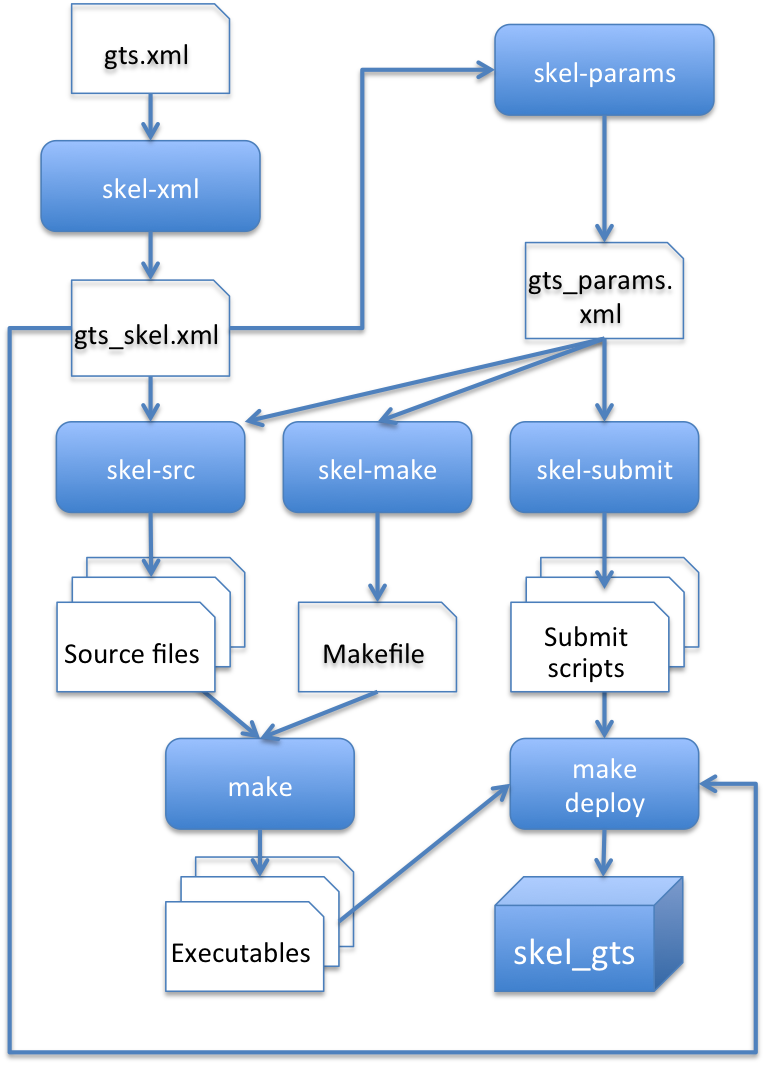
\includegraphics[width=75mm]
  {figures/overview.png}}
  \caption{\label{fig:overview} Skel Workflow}
\end{figure}

%Figure 1: Skel Workflow

At this point, the commands {\it skel source}, {\it skel makefile}, and {\it skel submit}
may be used to generate the source files, Makefile, and submission scripts that
comprise the skeletal application. With all of the components of the skeletal
application created, it is now time to build the application, using {\it make}, and
finally deploy the application to a directory from which it may be launched,
using {\it make deploy}, which copies the gts\_skel.xml file, executable files, and
submission script. The user now has a ready to run I/O benchmark without
having written any source code at all.



\section{Detailed Example of Manual Benchmark Creation}
In this section we will describe the steps used to create an I/O Kernel based
on the GTS application. The ADIOS config file for GTS can be found in the
examples directory.

The steps are

{\tt skel xml gts}

{\tt skel params gts}

Edit the parameters file, particularly the values of scalars that control array sizes,
and the desired tests to run.

{\tt skel makefile gts}

{\tt skel source gts}

{\tt skel submit gts} (optional)

{\tt make}

{\tt make deploy} (optional)



\section{Recreating a Run Using Skel Replay (Experimental)}
We have added a feature in this release that allows a benchmark to be created
automatically based on an existing bp file. This replay feature eliminates the
tedious nature of creating and tweaking a parameter file, instead taking that 
information directly from the bp file, settings file, or command line, in order
to allow direct replay while simplifying the steps that a user must take.

To show the usage of the replay feature, assume we have a bp file, out.bp,
that was produced by an application called myapp. Generating a benchmark based on out.bp is simple: 

{\tt skel replay myapp -b out.bp}

This single command generates an adios XML file, source code, a makefile, and a submission script, and finally executes the makefile, providing a ready to run benchmark.

\section{Using Skel for a remote replay (Experimental)}

In the case where you have a large bp file representing an I/O pattern you want to run
on a different machine, it may be desirable to extract the metadata information from the
bp file, rather than transferring the entire file to the remote machine. To
accomplish this, simply use the skeldump command as follows:

{\tt skeldump out.bp > out.yaml}

Skeldump creates a yaml file containing all of the information required to build the
benchmark on the remote machine. After moving only the yaml file to the remote machine,
the benchmark creation can be accomplished with:

{\tt skel replay myapp -y out.yaml}



\chapter{Skel Command Reference}

Most skel commands are of the form:
skel
subcommand project
\section{Available Subcommands}

\begin{description}
  \item[skel install] \hfill \\
Usage:

{\tt skel install}
  \item[skel makefile] \hfill \\
Generates a Makefile fit for building and deploying the skeletal
application.

Requires <project>\_skel.xml and <project>\_params.xml

Usage:

{\tt skel makefile <project>}
  \item[skel params] \hfill \\
Generates a parameters file that can be customized by the user.
Note that this command creates a file called <project> params.xml.default
so as to avoid overwriting a customized parameters file. This means that
the user should copy this file to <project> params.xml and edit before
proceeding with code generation.

Requires <project>\_skel.xml

Usage:

{\tt skel params <project>}
  \item[skel replay] \hfill \\
Generates a C or Fortran code that performs the I/O operations
described by the given bp file or yaml file.

Usage:

{\tt skel replay <project> -y <yaml\_file>}

{\tt skel replay <project> -b <bp\_file>}
  \item[skel source] \hfill \\
Generates a C or Fortran code that performs the I/O operations
described by the XML descriptor and the parameters file.

Requires <project>\_skel.xml and <project>\_params.xml

Usage:

{\tt skel source <project>}
  \item[skel submit] \hfill \\
Generates a submission script for the skeletal application

Requires <project>\_skel.xml and <project>\_params.xml

Usage:

{\tt skel submit <project>}

  \item[skel xml] \hfill \\
Generates the <project>\_skel.xml file.

Requires <project>.xml

Usage:

{\tt skel xml <project>}
\end{description}

\section{Skel Utilities}
\begin{description}
  \item[skeldump (experimental)] \hfill \\
Extracts necessary metadata from a bp file to create a skeletal application.
Metadata is produced in yaml format, and is sent to standard out.

Usage:

{\tt skeldump <bpfile> > <yamlfile>}

\end{description}


\chapter{The Parameters File}
Generation of a skeletal application requires some more information that is
found in the ADIOS configuration file. To specify this additional information,
the user must supply a Skel parameters file. The parameters file is an XML file
which contains the elements described in the following section.
Although it not overly dicult to construct your own parameters files, users
may find it more convenient to use the {\it skel params} command to automatically
generate a parameters file with default values, then simply edit the file to provide
the desired configuration.
\section{Elements}
\begin{description}
  \item[<skel-config>] \hfill \\
Each parameters file must contain exactly one
<skel-config> element as the only element at the root level of the document. The
<skel-config> element should contain one <adios-group> element and one <batch>
element, as described below.

{\it Supported Attributes:}
  \begin{description}
    \item[application]
The name of the application described by the document.
This should correspond to the project used for the skel calls, and
the name of the original XML file given to skel xml .
  \end{description}


  \item[<adios-group>] \hfill \\
The <adios-group> element is a child of the root <skel-config>
element. It corresponds to the adios-group that will be written by the I/O
skeletal application being generated. The <adios-group> element contains a collection of
<scalar> and <array> elements corresponding to the variables described for the group
in the ADIOS config file.

{\it Supported Attributes:}
  \begin{description}
    \item[name]
The name of the ADIOS group that this element describes
  \end{description}


  \item[<scalar>] \hfill \\
Represents a scalar variable that is described in the ADIOS descrip-
tor. Often integer valued scalars will be used to determine the dimensions
of arrays, thus providing appropriate values is essential for creating mean-
ingful benchmarks.

{\it Supported Attributes:}
  \begin{description}
    \item[name]
The name of the scalar variable
    \item[type]
(Optional) The type of this variable in the generated code. Supplied
for convenience by skel params .
    \item[value]
A value, of the proper type, that will be assigned to this scalar
variable in the generated code.
  \end{description}

  \item[<array>] \hfill \\
Represents an array variable that is described in the ADIOS descrip-
tor.

{\it Supported Attributes:}
  \begin{description}
    \item[name]
The name of the array variable
    \item[type]
(Optional) The type of this variable in the generated code. Supplied
for convenience by {\it skel params}.
    \item[dimensions]
(Optional) A list of the scalar values that will be used to
determine the dimensions of this array
    \item[fill-method]
Determines how the array memory will be initialized in the
generated code
  \end{description}
  \item[<batch>] \hfill \\
Describes a set of tests to be performed by the generated I/O kernel.
The <batch> element contains one or more <test> elements.

{\it Supported Attributes:}
  \begin{description}
    \item[name]
The name of the batch. Used to name the submission script and
other elements of the batch job.
    \item[cores]
The number of MPI tasks that will be used for the skeletal application
    \item[walltime]
Amount of runtime requested by the generated submission script
  \end{description}
  \item[<test>] \hfill \\
Describes a single test to be performed.

{\it Supported Attributes:}
  \begin{description}
    \item[type]
The type of test to be performed. Currently only write is supported.
    \item[group]
The ADIOS group to be written
    \item[method]
The ADIOS write method to use for writing (i.e. POSIX). A
full listing of available methods can be found in the ADIOS manual.
    \item[iterations]
The number of times to repeat this test
    \item[rm]
determines whether and when to remove the written output files. One
of \{pre, post, both, none\}
  \end{description}
\end{description}



\chapter{Yaml File Format}

Skel supports various methods for specifying the high-level I/O description to be
used for creating skeletal applications. One of these is the yaml file, described below.
YAML is a data serialization language that is similar
to JSON. YAML supports data abstractions including sequences and mappings, and allows
these to be nested. General information about YAML is available at http://www.yaml.org/

The yaml format described here is the one that is produced by the {\tt skeldump} utility,
and which is accepted by the {\tt skel replay} command, both described elsewhere in
this manual.
\vspace{5mm}

At the top level of the yaml file, there are a series of mappings as follows:
\begin{description}
  \item[lang] specifies the target language, currently C and fortran are supported.

  \item[procs] indicates the number of MPI tasks involved in the I/O operations.

  \item[group] is the name of the ADIOS group in which to write the variables.

  \item[variables] is a sequence of mappings representing the variables to be written

\end{description}

\vspace{5mm}
Each variable is represented by a nested mapping that consists of:
\begin{description}

  \item[name] The name of the variable

  \item[type] The unit type of the variable, should correspond to a valid type in the target language

  \item[dims] Either {\tt scalar}, or a comma separated list of array dimensions

  \item[value] (For scalars) a string representing the value to be assigned to this variable in the skeletal application code.

\end{description}






\chapter{Skel Settings File}
Skel provides a collection of configurable options which are exposed in the
Skel settings file. The settings file is located in the user's home directory at
/.skel/settings.
The settings file consists of single line entries of the form
<name>=<value>.
Blank lines and lines starting with \# are ignored. Entries in the settings files are
case sensitive, and lower case is typically used for all names and yes/no values.
\section{Available Settings}
\begin{description}
  \item[deploy\_dir]
This is the directory into which the compiled applications will be
copied to be executed. This directory should be visible to the compute
nodes.
  \item[submit\_target]
This determines which submission script template will be used
by
skel submit
. Templates for
jaguar
and
sith
are included in this
release.
  \item[sleep\_before\_open (yes/no)]
Determines whether a short
sleep
statement is
inserted in the code before the
adios
open
call. Default is
no
.
  \item[barrier\_before\_open (yes/no)]
Determines whether an
MPI
Barrier
call is
inserted into the generated code before
adios
open
. Default is
yes
.
  \item[barrier\_before\_access (yes/no)]
Determines whether an
MPI
Barrier
call is
inserted into the generated code before the sequence of
adios
write
calls.
Default is
no
.
  \item[barrier\_before\_close (yes/no)]
Determines whether an
MPI
Barrier
call is
inserted into the generated code before
adios
close
. Default is
no
.
  \item[barrier\_after\_close (yes/no)]
Determines whether an
MPI
Barrier
call is in-
serted into the generated code after
adios
close
. Default is
no
.
  \item[barrier\_after\_steps (yes/no)]
Determines whether a single
MPI
Barrier
call
is inserted into the generated code after the nal
adios
close
. Default is
no
.
  \item[use\_adios\_timing (yes/no)]
Determines whether a call is inserted to output
detailed timing information collected by ADIOS. For this to work, your
adios distribution must have been configured using
--enable-skel-timing
.
Default is
no
\end{description}





\chapter{Low-Level Timing Mechanism}
By default, applications generated by skel will produce a summary timing re-
port, sending it to standard out. On most platforms, this will be captured in
the output file produced by the job script. The summary report contains tex-
tual information about the overall time taken by the various I/O operations. If
more detail is desired, ADIOS has a mechanism for gathering low-level timing
information for various events that occur within the ADIOS I/O calls.

\section{Using the Low-Level Timing Mechanism}
To use the low-level timing mechanism, you must use an ADIOS library that has
been built with this low-level timing mechanism enabled. Simply build ADIOS
as described in the ADIOS manual, inserting
--enable-skel-timing
in the
configure
command. We do not recommend enabling the low-level timing
mechanism while running production codes.
Once you have enabled low-level timing in ADIOS, you only need to enable
generation of low-level timing calls in your Skel settings file. This is done by
including the line:
{\tt use\_adios\_timing=yes}
in your Skel settings file. This will
cause the
skel source
command to include an additional call near the end
of the generated skeletal application to output the detailed timing information
that has been collected. The detailed timing information is written to a separate
file using XML. This will work best if used to write a single iteration of a single
group.
The low-level timing mechanism provides detailed timing information for
only some of the available write methods. As of this release, the supported
methods are
POSIX
,
MPI
LUSTRE
, and
MPI
AMR
.
\section{Extracting Timing Information}
The XML file that is produced by ADIOS contains a large amount of measure-
ment data, but it is somewhat unwieldy to work with directly. So, we have
included an additional utility,
skel
extract.py
, which allows data from the
XML file to be exported as a CSV file that is simple to load using tools such as R or Matlab.



\chapter{Hints for Porting Skel}
Skel has been developed and tested on only a small handful of platforms. While
we expect most functionality will be portable to a wider range of machines,
there are likely to be some issues arising when running skel on your system.
There are a few hints in the following sections that may help you to get started.
If further assistance is needed to get skel working, please contact lot@ornl.gov.

\section{Makefiles}
Assuming that they work properly, Makefiles generated by skel are quite conve-
nient, as the skel user need not think about how to compile the code, but can
simply type make. All of the details are taken care of by skel. We have tested
skel on only a few systems at this point, and thus it is quite possible that the
Makefile generated by skel may fail on some systems. Users familiar with make
with a need to adjust some aspect of the generated makefiles should investigate
/.skel/templates/Makefile.default.tpl. This template file is used by Skel to
generate Makefiles, and can be adjusted to the needs of the user. The template
syntax is simple, with {\tt \$\$VAR\_NAME\$\$} used to indicate template substitutions
to be made by skel makefile. Again, if you run into trouble with this, please
contact us as described above.

\section{Submission Scripts}
Similar to the Makefile generation, skel uses templates to generate submission
scripts for the generated applications. The submission templates are also located
in
/.skel/templates/, and are named submit <target>.tpl, where <target>
corresponds to the submit target defined in the user's settings file. To create a
new submit target , simply copy one of the existing template files, and rename
it with the desired submit target name. Then, adjust the submission syntax
so that the generated files work properly with the submission mechanism on
your system. Once again, if you run into trouble with this, please contact us as
described above.


\end{document}





